%$Header: /usr/u/rz/AMBook/RCS/intro.tex,v 1.1 1992/02/13 22:47:39 rz Exp rz $
\chapter{Introduction}

Algebraic manipulation is the study of algorithms for manipulating
mathematical quantities.  What distinguishes it from other areas of
mathematical computation is the attention paid to accurately modeling the
mathematical semantics of the objects being manipulated.  The first
manifestation of this is that while conventional computation systems define
an integer to be a whole number with absolute value less then $2^{31}$ or
$2^{63}$ typically, algebraic manipulation systems define integers to be
whole numbers, with no limit set to their size.  Though this distinction
makes little difference in many computations, algebraic manipulations
focuses on those techniques and problems where exactness or the ability to
model a complex mathematical concept is important.

This book discusses the basic algorithms for manipulating mathematical
quantities and how they are implemented.  Mathematical quantities divide
into two basic types, exact and inexact.  Among the exact quantities are
rational integers, algebraic numbers, polynomials, differential forms and
vector fields.  Inexact quantities include truncated power series and
Fourier series, and continued fractions.  Computing with these types of
quantities instead of floating point numbers and fixed precision integers,
yields three benefits.  First, the computation can take place exactly. Thus
if successful, one can prove than an answer is exactly $\sqrt{3}$ or
$1/137$ not just that it is close to these values.  Second, symbolic
quantities represent an entire function, not just its value at a point.
This allows more global information about the behavior of a system to be
determined.  Finally, symbolic quantities can represent and manipulate
mathematical abstractions that are not usually considered part of
computational mathematics, like rings, ideals, Riemann surfaces and
homology groups.

This book discusses the algorithms for performing symbolic
mathematical calculations.  We will be dealing not only with large
integers, but with algebraic numbers, polynomials and transcendental
functions.  Systems with these capabilities are often called {\em
algebraic manipulation} systems and the field we will be studying is
called {\em algebraic manipulation\/}, {\em computer algebra} or {\em
symbolic computation}.  For example, an algebraic manipulation system
could take an expression like
\[
S = \sin^2 x + \cos^2 x
\]
differentiate it to get
\[
2 \sin x \cos x + 2 \cos x \, (- \sin x) = 0.
\]
From this it is clear that $\sin^2 x + \cos^2 x$ is a constant.  To
determine to which constant $S$ is equal, we ask the system to evaluate $S$
at $\pi$:
\[
\sin^2 \pi + \cos^2 \pi = 0^2 + (-1)^2 = 1.
\]
Notice that the value of $\cos \pi$ is exactly $1$---there is no round
off error and it is not
$1.00000\pm\epsilon$. Thus $\sin^2 x + \cos^2 x = 1$.  This is a trivial
example of one of the ways algebraic manipulation systems can be used to
solve problems.

Current algebraic manipulation systems have been designed to perform long
tedious calculations that, at one time, were the responsibility of graduate
students.  They can compute integrals, factor polynomials and develop power
series expansions.  They are called upon to solve differential equations
and invert matrices.  At one time all of the calculations performed by
algebraic manipulation systems were exact, although now approximation
techniques are proving to be very valuable.  Truncated power series and
arbitrary precision floating point calculations are often provided and have
been useful.  Even conventional floating point techniques are being used in
a mixed mode of computation, part of the calculation being numeric and part
being symbolic.

\medskip

Here we outline the basic algorithms and techniques algebraic manipulation
systems use to perform calculations.  We do not attempt to describe how
these systems are used to solve real problems.  But we feel that by
understanding the mechanisms used, it will be far easier to understand the
limitations and capabilities of algebraic manipulation systems.

\section{A History of Symbolic Systems}

Algebraic manipulation has a history nearly as old as mechanized
computation itself.  The first mention of symbolic computation is in
the following quote of Lady Ada Augusta, Countess {\Lovelace},
describing the capabilities of {\Babbage}'s analytical engine.

\begin{quotation}
Many persons who are not conversant with mathematical studies imagine that
because the business of [Babbage's Analytical Engine] is to give its
results in numerical notation, the nature of its processes must
consequently be arithmetical and numerical rather than algebraic and
analytical.  This is an error.  The engine can arrange and combine its
numerical quantities exactly as if they were letters or any other general
symbols; and in fact it might bring out its results in algebraic notation
were provisions made accordingly.
\end{quotation}

The first modern program to perform algebraic computations was a
differentiation program developed for the Univac I by {\Kahrimanian}in
1953 \cite{Kahrimanian1953-gs} and {Nolan} \cite{Nolan1953-te}.  
In this program, expressions were
represented as linearized binary trees.  The user's input would be
indicated in essentially the same manner; no parser for mathematical
expression was provided.  Though this program was not usable anyone
other than the author, it was one of the first demonstrations that
computers could be used for other than numerical computation.

The next significant step in the development of algebraic systems was
the creation of the programming language {\Lisp} by John {\McCarthy}
\cite{McCarthy1960-bz,McCarthy1969-af}, then of MIT.  According to certain
traditions {\McCarthy}'s image of what a differentiation program should
look like was the model for how {\Lisp} should work
\cite{McCarthy1960-op}.\footnote{For a more detailed
discussion of the early history of {\Lisp} see \cite{Stoyan1984-fn}.}
Perhaps the second commonest {\Lisp} program ever written is one for
differentiation---certainly factorial rates first.  For many years
virtually all computer algebra systems were built on top of {\Lisp}.  Although
several of the mechanisms popularized by {\Lisp} are extremely valuable in
computer algebra systems, in particular automatic storage management, {\Lisp}
is no longer essential for building computer algebra systems.

Given that the first {\Lisp} program was for differentiation and there
did not appear to be an algorithm for the inverse problem, it was
natural to anti-differentiation or integration as a test for the new
techniques of Artificial Intelligence being developed at the AI group
at MIT.\index{Artificial Intelligence Laboratory, MIT} Thus not long
after the first {\Lisp} system was operational, one of Marvin
Minsky's\footnote{Along with John {\McCarthy}, Marvin {\Minsky} founded the
Artificial Intelligence group of the Research Laboratory for
Electronics at MIT.  Later this group became the Artificial
Intelligence Group at Project Mac and then the Artificial Intelligence
Laboratory at MIT.  John {\McCarthy} left in the early sixties to form
the Stanford Artificial Intelligence Laboratory.\index{Artificial
Intelligence Laboratory, Stanford}} students, James {\Slagle},
developed a program for integration.  {\Slagle}'s integration program
was called {\Saint} and was completed in 1962 \cite{Slagle1963-dt}.
{\Saint} produced admirable results; it was about equal to a freshman
calculus student in skill though perhaps a little quicker.  Slagle's
program was not based on a mathematical understanding of the
integration problem.  Instead it contained a table of known integrals
and collection of transformations between integrals, such as
integration by parts.  It then used heuristics to guide the
application of the transformations.  {\Saint} tended to wander in a
rather aimless fashion and would often take a great deal of time to
solve a problem.  Despite its short-comings {\Saint} drew a great
deal of attention to the integration problem and to related problems
in artificial intelligence.

At about this time, the early sixties, a number of groups began to
seriously build general systems that would make computerized symbolic
mathematical computation available to non-programmers.  One of the early
systems was a collection of assembly language routines called {\Alpak}
\cite{Brown1963-wx,Brown1964-cs} developed at Bell Laboratories.  {\Alpak}
allowed the user to manipulate polynomials and rational functions
easily, and provided routines for differentiating, multiplying,
dividing, and other operations.  Later the {\Alpak} routines were
combined with an reasonably natural user language for specifying the
operations, and ultimately this system evolved into {\Altran}
\cite{Brown1973-gv}.  {\Altran} was developed intensively during the
late sixties and was widely used in the early seventies.  The
{\Altran} group was led by W.~S.~{\BrownWS} and included
S.~I.~{\Feldman}, W.~M.~{\Gentleman}, A.~D.~{\HallA}, S.~C.~{\JohnsonS},
M.~D.~{\McIlroy} and D.~M.~{\Ritchie}, many of whom later contributed
to the development of Unix.  The {\Altran} group was responsible for
many important early advances in algebraic manipulation: the modular
greatest common divisor (GCD) algorithm, the heap multiplication
algorithm and the use of factored form to represent polynomials.

At IBM, a group led by Jean Sammet developed {\Formac}
\cite{Sammet1964-wt,Tobey1965-mo} for the IBM 7090.  Unlike
{\Alpak} and {\Altran}, {\Formac} was not designed to deal exclusively
with polynomials and rational functions.  It used a tree-like
structure similar to that adopted by {\Kahrimanian}, {\McCarthy} and
{\Slagle}, which allowed transcendental functions to be used as easily
as polynomials and rational functions.  When originally released, the
algorithms used in {\Formac} were not nearly as efficient as those in
{\Altran}.  This, coupled with the more general representation chosen,
caused {\Formac} to be substantially slower than some of the other
systems at the time.\footnote{Some of these efficiency problems were
resolved by Knut {\Bahr} and {\Hulzen} \cite{Bahr1974-cv,Bahr1974-bl,Van_Hulzen1974-ab} 
who went to great lengths to improve
and enhance the system.} {\Formac} was implemented as a collection of
subroutines like {\Altran}, but its user interface was somewhat novel.
A preprocessor would convert Fortran code, which had {\Formac}
statements embedded, into conventional Fortran with the
{\Formac} statements converted to appropriate sequences of function
calls. In the late sixties, the Fortran preprocessor was converted to a
PL/I preprocessor and the system rewritten for the IBM 360.  This approach
made all of the control structures and facilities of the host language
available to the algebraic manipulation user, whereas in {\Altran} only those
facilities provided by the {\Altran} language could be used.

At the University of Wisconsin at Madison, George {\Collins} developed
PM, a polynomial manipulation system that used reference count system
to manage its storage.  This was later supplanted by \Sac-1, another
collection of Fortran callable routines for manipulating polynomials.
The development of these systems was motivated by the quantifier
elimination methods for the elementary theory of real closed fields
discovered by {\Tarski} \cite{Tarski1951-qv}, {\Seidenberg} \cite{Seidenberg1954-tu} and {\CohenP} \cite{Cohen1969-lw}.  The computer algebra required to
implement these algorithms depended heavily on computing polynomial
resultants and greatest common divisors and isolating real roots of
polynomials.  {\Collins}' group was instrumental in developing some of
the powerful, modern algorithms for dealing with these problems.

\smallskip

In the late sixties a number of researchers developed algebraic
manipulation systems that would allow the engineer or scientist to use
the system in a more natural manner than allowed in the earlier
systems.  At the Massachusetts Institute of Technology, Carl
{\Engleman} developed {\Mathlab}, which was designed to be an
interactive aid in solving problems using algebraic manipulation.  In
contrast to systems like {\Sac} and even {\Altran}, {\Mathlab} was
intended to be used as an interactive symbolic calculator, available
for quick, relatively simple, computations that might take an engineer
a few hours to do by hand, but which could be performed by a computer
in a few minutes.  Among the key ideas of {\Mathlab} found in later
systems are two dimensional output of mathematical expressions on
character based terminals and the use of general purpose
representation for many operations, which allowed the system to deal
with summations matrices and other structures not allowed in earlier
systems.  In addition, {\Mathlab} allowed the use of a special
polynomial representation for speed when appropriate.  Among those who
worked on {\Mathlab} are S.~{\BloomS}, C.~{\Engleman},
B.~W.~{\Diffie}, W.~A.~{\MartinW}, M.~{\Manove} and J.~{\MosesJ}.
{\Mathlab} is written in {\Lisp}.

At Stanford, Tony {\Hearn} was developing a system for performing
computations in quantum electrodynamics.  He realized that his system
could be applied more generally than just quantum electro-dynamics
calculations, so he refined his system to be, what is now called
{\Reduce} 3.  {\Reduce} was also designed to be a desk calculator type
of system with interactive input and two dimensional output and it
built on many of the ideas in {\Mathlab}.  One of the main design
goals of the Reduce group was portability to a large number of
different machines.  As a consequence the system was built on a
relatively small core of {\Lisp} functions.  The core has evolved into
what is now called Portable Standard Lisp (PSL)\index{Lisp! Portable
Standard} \cite{Marti1980-og}, which has been implemented on a large
number of different machines.  This allows {\Reduce} 3 to run a large
number of different types of machines, more than most other algebraic
manipulation systems.  Currently it is one of the most widely
distributed systems.

In the late sixties, David {\BartonDRa} of the University of
Cambridge, England, was trying solve the ``main problem of the lunar
theory'' using Delaunay's approach using Poisson series (which are
related to Fourier series).  To aid in his work he had developed a
simple system for manipulating Poisson series.  In 1968, {\BartonDRa},
together with Steve {\Bourne} (later of Unix fame) and John {\Fitch},
began the development of {\Camal} \cite{Fitch1975-sn}, a general purpose
algebraic manipulation system that was particularly tuned for
performing the Poisson series calculations that are required by
celestial mechanics problems.  {\Camal} was originally written in
assembly language for the ATLAS, and was then rewritten in BCPL.

At the end of the sixties efforts began on the development of systems that
were to be highly interactive, utilized the most modern and efficient
algorithms and which were capable of any of the computations performed by
the systems mentioned above.

Perhaps the best know algebraic manipulation system is {\Macsyma}, which
was developed at MIT from the late sixties and till about 1982.  In
\sectref{Macsyma:Intro:Sec} we give a detailed introduction to
{\Macsyma} and in \sectref{Quantum:Ex:Sec} an example of using
{\Macsyma} to solve a real problem is presented.  Among those active
in its development at MIT are D.~R.~{\BartonDRb}, R.~J.~{\Fateman},
M.~R.~{\Genesereth}, J.~P.~{\Golden}, J.~L.~{\Kulp}, W.~A.~{\MartinW},
J.~{\MosesJ}, B.~M.~{\Trager}, P.~S.-H.~{\WangP}, D.~Y.~Y.~{\Yun} and
R.~E.~{\Zippel}.

The Scratchpad system was developed by J.~{\Griesmer} and R.~D.~{\Jenks} in
the early seventies.  It was an amalgam of several different systems,
including much of the code used in {\Mathlab}, as well as {\MosesJ}' SIN
and some of {\MartinW}'s code.  In the middle 70's the Scratchpad group
realized that a fundamental problem limiting further development was
an appropriate language for describing algebraic algorithms.
Influenced by earlier work of Dave {\BartonDRb}, Dick {\Jenks} and Barry
{\Trager} developed Axiom \cite{Jenks1992-cu}, which incorporates a new
language for describing mathematical algorithms.

\index{SMP} \index{Ashmedai}
Recently, a number of algebraic manipulation systems have been made
commercially available.  Among the more notable ones are {\Mathematica}
\cite{Wolfram1988-cy}, developed by Wolfram Research Inc. primarily for
calculations in high energy physics, {\Maple} \cite{noauthor_1987-fl},
developed at the University of Waterloo, and Deriv which runs on IBM
PC's.\rightmarginnote{need much more on Mathematica, Maple and Scratchpad.}

In addition there have been several special purpose system, like Ashmedai
\cite{Levine1976-pq} that have been used for specific calculations.

\section{Examples of Algebraic Manipulation}
 
Before discussing the algorithms of algebraic manipulation, it would be
beneficial to have some experience in using an algebraic manipulation
system.  The following sections describe {\Macsyma}, one of the most extensive
algebraic manipulation systems, and give some examples of its use.

\subsection{Introduction to Macsyma}
\label{Macsyma:Intro:Sec}

{\Macsyma} is a very large interactive system that possesses many of the
raw computational faculties of a graduate student, but that follows
directions better, complains less and is usually faster and more accurate.
It was designed to be a computational aid to mathematicians, scientists and
engineers, to be used in much the same way that pocket calculators are used
today.  Among the facilities {\Macsyma} has at its disposal are routines for
calculating derivatives, integrals, Taylor series, Poisson series, Laplace
transforms and factorizations of polynomials.  There also exist routines
for computing with exact rational numbers and floating point numbers of any
specified precision and for obtaining both two and three dimensional
projective plots of functions.

The original design of the {\Macsyma} system was laid out by Carl Engleman,
William A.  {\MartinW} and Joel {\MosesJ} in 1968, while working at the
Massachusetts Institute of Technology's Project MAC.  They built on their
previous experience with the {\sc Mathlab} '68 system and the theses of
{\MartinW} and {\MosesJ}.  {\MartinW}'s thesis discussed the construction of an
algebraic manipulation system to solve certain problems in applied
mathematics.  This system was designed to show how easy to use such a
system could be \cite{Martin1967-uz}.  It made use of a graphics display
and light pen to display formulae in two dimensions and to allow easy
specification of subformulae.  {\MosesJ} developed a program (SIN) that was
able to perform indefinite integrals about as well as a typical graduate
student \cite{Moses1968-oq}.  His thesis was one of the first where more
sophisticated mathematics replaced heuristic techniques.  It was
significantly more powerful than {\Slagle}'s work.  In addition, they relied
on an earlier program developed by Korsvold \cite{Korsvold1966-ja,Korsvold1965-ml} at Stanford's Artificial Intelligence
Laboratory\index{Artificial Intelligence Laboratory, Stanford} for simplifying
algebraic expressions, and on the ideas in a two dimensional display
program for mathematical formulae developed by Millen \cite{Millen1968-wc}.
Nearly all these capabilities were rewritten in the first version that
could be used to solve real problems ({\em circa} 1971).

{\Macsyma} was under continuous development at MIT till about 1982.
During this period the developers made a number of contributions to the
field of algebraic computation.  {\Macsyma} was the first general purpose
system to implement the Risch algorithm for integration of elementary
functions, it had the first package for evaluating definite integrals
symbolically and it had the first package for computing limits.  During
the seventies {\Macsyma}'s developers produced many important results in
computer algebra, among which where the first multivariate polynomial
factorization package, practical algorithms for integration of algebraic
functions, probabilistic algorithms for polynomial manipulation,
algorithms for summing infinite series and algorithms for manipulating
hypergeometric functions.

Until 1982 nearly all {\Macsyma} users used a special ``{\Macsyma} Computer''
at MIT.  This machine was relatively fast, had a huge memory for the period
(about 1 megabyte), and was one of the few machines that was both
configured to run a symbolic computation program efficiently and devoted to
performing symbolic computation.  Since then, the changing economics of
computers have made it possible for computer algebra systems to run on much
less expensive machines.  Now there are several groups building computer
algebra systems, several of which can run on personal computers.  (Even
{\Macsyma} has been made to run on an IBM PC/AT.) In 1982 {\Macsyma} was sold
to Symbolics, Inc.  who currently markets it.\footnote{Symbolics, Inc.
currently supports and markets {\Macsyma} on a variety of different machines.
{\Macsyma} is also available to US government agencies and contractors through
the Department of Energy Software Clearinghouse.}

In the following paragraphs we give a short demonstrations of {\Macsyma}.
These examples were originally produced by Richard {\Fateman} around 1971, but
have been modified somewhat since then.
 
\begin{verbatim}
(C1) X/(X^3+1);
                                      X
(D1)                                ------
                                     3
                                    X  + 1
\end{verbatim}
When {\Macsyma} is started it gives an introductory greeting (which varies
from machine to machine) and prints {\tt (C1)} to indicate
it is ready to go to work.  The user types in his expressions in the
same format as is used in many programming languages.  An ``{\tt *}''
is used to represent multiplication.  Expressions are terminated by
a ``{\tt ;}''.  The expression which has been typed is then
simplified somewhat and printed in the conventional mathematical notation.
This value is assigned to the variable {\tt D1}.  If you do not want to
see the {\tt D}-line, then expression may be terminated by a ``$\$ $'' (dollar
sign) instead of a semi-colon.  In either case a {\tt D}-line is
produced.  Notice that no value was
assigned to {\tt X}.  The ability to deal with these symbolic variables or {\em
atoms} is one of the main features that distinguishes algebraic manipulation
systems from other forms of mathematical computation.

Most implementations of algebraic manipulation systems are designed to
display their results using character oriented displays.  (This is a
trend that will disappear soon.)  As a consequence, when actually using an
algebraic manipulation system, one will be faced with something very similar to
what appears above, which is relatively difficult to read.  For
readability sake, we will present the results of {\Macsyma}'s
calculations using conventionally typeset formula.  {\Macsyma}'s input, however, will continue to be
given in a keyboard style.

\begin{verbatim}
(C2) %+%;
\end{verbatim}
\mdline{\frac{2 x}{x^3 +1}}{D2}
A percent sign is used to represent the value of the last {\tt D}-line (which
we are showing typeset, 
\begin{verbatim}
(C3) SIN(X);
\end{verbatim}
\mdline{\sin x}{D3}
\begin{verbatim}
(C4) SIN(X-%PI/2);
\end{verbatim}
\mdline{- \cos x}{D4}
The elementary functions may be typed in the conventional manner.  Notice that
{\tt\%PI} is used to represent $\pi$.  Similarly {\tt\%E} is used to represent
the base of natural logarithms, and {\tt\%I} is used to represent $\sqrt{-1}$.
The simplifier does change the expression typed when certain ``obvious'' changes
are indicated.
\begin{verbatim}
(C5) (X+3)^20;
\end{verbatim}
\mdline{(x+3)^{20}}{D5}
Sometimes it is not ``obvious'' that a simplification is desirable.
In the example above the expression is not expanded.  There is however
a routine which does expand polynomials (as well as a number of other
things) called {\tt RATSIMP}.  {\Macsyma} provides a number of other
special purpose simplifiers. After a bit of experience, it is not hard
to see which one is appropriate at a given time.
\begin{verbatim}
(C6) RATSIMP(%);
\end{verbatim}
\mdline{
  \begin{aligned}
    x^{20} &+ 60 x^{19} + 1710 x^{18} + 30780 x^{17} + 392445 x^{16}
 + 3767472 x^{15}\\
    & + 28256040 x^{14} + 169536240 x^{13} + 826489170 x^{12} + 3305956680 x^{11}\\
    &+ 10909657044 x^{10} + 29753610120 x^9 + 66945622770 x^8 \\
    & + 123591918960 x^7 + 185387878440 x^6 + 222465454128 x^5 \\
    &+ 208561363245 x^4 + 147219785820 x^3 + 73609892910 x^2 \\
    &+ 23245229340 x + 3486784401
  \end{aligned}}{D6}

Arbitrary size integers can be used, limited only by the storage
capacity of the machines on which {\Macsyma} is run.  In {\Macsyma}'s case this
facility is provided by the underlying {\Lisp} implementation, but is an
expected part of all computer algebra systems.  Similarly, floating
point numbers of virtually any precision can also be used.

As an example consider $e^{\pi \sqrt{163}}$, which was declared to be an
integer in an April fool's issue of {\em Scientific
American\/}.\rightmarginnote{What year?}

\begin{verbatim}
(C7) %e^(%pi*sqrt(163))$
\end{verbatim}
The {\Macsyma} function {\tt BFLOAT} causes its argument to be evaluated
to the numerical precision specified by the variable {\tt FPPREC}.  Thus
\begin{verbatim}
(C8) BFLOAT(D3),FPPREC=30;
(D8)       2.62537412640768743999999999999B17
\end{verbatim}
Which is pretty close to the integer $262537412640768743$.  However, when
computer to forty digits we have:
\begin{verbatim}
(C8) BFLOAT(D3),FPPREC=40;
(D8)  2.625374126407687439999999999992500725972B17
\end{verbatim}

Returning to the polynomial on line {\tt D6}, we can differentiate it using
the function {\tt DIFF}.
\begin{verbatim}
(C10) DIFF(D6,X);
\end{verbatim}
\mdline{
  \begin{aligned}
20 x^{19} &+ 1140 x^{18} + 30780 x^{17} + 523260 x^{16} + 6279120 x^{15} \\
& + 56512080 x^{14} + 395584560 x^{13} + 2203971120 x^{12} \\
& + 9917870040 x^{11} + 36365523480 x^{10} + 109096570440 x^9\\
& + 267782491080 x^8+ 535564982160 x^7 + 865143432720 x^6 \\
&+ 1112327270640 x^5 + 1112327270640 x^4 + 834245452980 x^3\\
& + 441659357460 x^2 + 147219785820 x + 23245229340
\end{aligned}}{D10}

\noindent
The validity of this result can be checked by factoring {\tt D10}.
\begin{verbatim}
(C11) FACTOR(D10);
\end{verbatim}
\mdline{20 (x+3)^{19}}{D11}
The {\tt FACTOR} command is one of the most sophisticated in
{\Macsyma}.  It does not proceed by trial and error, but rather uses an algorithm
that will produce a factorization of a polynomial into irreducible
polynomials.  If {\tt FACTOR} does not return a factorization, the input
is guaranteed to be irreducible as a polynomial over the integers.  The
algorithm used is discussed in more detail in later sections.

The uses of factorization in number theory, algebraic coding theory
factor and for solving algebraic equations are clear.  What is
surprising to many new users of algebraic manipulation systems is just
how useful it can be for simplifying expressions.  One example of this
is given a bit later when we deal with matrices and another is
contained in \sectref{Quantum:Ex:Sec}.
\begin{verbatim}
(C12) D2;
\end{verbatim}
\mdline{\frac{2x}{x^3 +1}} {D12} 
{\Macsyma} doesn't forget the answers it gave previously.  In addition
to being able to differentiate expressions it can integrate them too.
To do so it makes use of some of the heuristic ideas of Slagle's \cite{Slagle1963-dt} and
{\MosesJ}'s theses \cite{Moses1968-oq} and includes an
implementation of the \keyi{Risch algorithm}, which is described in
the later chapters.  Since the Risch algorithm is a \keyi{decision
procedure}, if the integration package fails on a problem (for which
the Risch algorithm is applicable) the integral is not integral in
terms of elementary functions.  For the problem given here,
\keyi{Hermite's algorithm} for integration of rational functions is
sufficient.
\begin{verbatim}
(C13) INTEGRATE(D12,X);
\end{verbatim}
\mdline{2 \left( \frac{\log \left(x^2-x+1\right)}{6} +
\frac{\arctan \frac{2 x - 1}{\sqrt{3}}}{\sqrt{3}} -
\frac{\log (x + 1)}{3} \right)}{D13}
The function {\tt LOG} is used to represent the natural logarithm function.
Notice that if a freshman calculus student were to write this expression
down, he would probably do two things.  First, he would get it wrong.  This
is one of the biggest advantages of algebraic manipulation systems.
Algebraic manipulation systems tend not to get tired, or lazy, or
sloppy.  Their answers are usually correct, though sometimes they are
answers to different questions than you thought had been asked.

The second difference between {\Macsyma} and our hypothetical calculus
student is that the students answer would probably be written differently.
The constant $2$ might be multiplied through or the logarithms could be
rearranged.  In fact it is likely that the student would consider 
\[
\frac{1}{3} \log \frac{x^2 - x + 1}{(x+1)^2} 
+ 2 \frac{\arctan \frac{2 x - 1}{\sqrt{3}} }{\sqrt{3}}
\]
to be a better simplified answer.  Producing a ``simplified'' result, one
that the user of the system can understand, is one of the most difficult
problems in computer algebra.  

We can check {\Macsyma}'s efforts by differentiating {\tt C13} and checking
to see if it matches {\tt D12}.
\begin{verbatim}
(C14) DIFF(D13,X);
\end{verbatim}
\mdline{2 \left(\frac{2}{3 \left( \frac{(2 x-1)^2}{3} +1 \right)}
 + \frac{2 x-1}{6\,(x^2 - x +1)} 
 - \frac{1}{3\,(x+1)}\right)}{D14}
The differentiation function took the derivative of each term in the
sum just as one would using the rules taught in calculus courses.
However, it doesn't simplify its results completely.  This again is an
example of the system simplifier performing the absolute minimum
amount of simplification necessary to return a reasonable answer.
Again, the {\tt RATSIMP} function may be used to combine terms and cancel
common factors from numerator and denominator.
\begin{verbatim}
(C15) RATSIMP(D14);
\end{verbatim}
\mdline{\frac{2 x}{x^3 +1}}{D15}

{\tt RATSIMP} returns the original expression, giving us some faith in
the integration package.  Though the default simplification routines
try to minimize the change that they make to the expression, {\Macsyma}
provides a large number of different simplifiers for dealing with the
different types of problems that arise.

\begin{verbatim}
(C16) TAYLOR(SIN(X),X,0,5);
\end{verbatim}
\mdline{x - \frac{x^3}{6} + \frac{x^5}{120} + \cdots}{D16}
Occasionally it is impossible to obtain an exact solution to 
a problem.  Then an applied mathematician often relies upon
power series techniques.  
The {\tt TAYLOR} command obtains a power series expansion for functions of
one or more variables.  The arguments to {\tt TAYLOR} in the usual one variable
case are the function to be expanded, the variable of expansion, the point of
expansion and the highest degree term to be retained.
\begin{verbatim}
(C17) TAYLOR(COS(X),X,0,5);
\end{verbatim}
\mdline{1 - \frac{x^2}{2} + \frac{x^4}{24} + \cdots}{D17}
{\tt TAYLOR} is aware of the expansions for all the familiar elementary
functions.
\begin{verbatim}
(C18) D16*D17;
\end{verbatim}
\mdline{x - \frac{2 x^3}{3} + \frac{2 x^5}{15} + \cdots}{D18}
The value returned by {\tt TAYLOR} uses a different internal representation
than the expressions we have encountered until now.  Taylor series may be
combined with general expressions and the result will also be a Taylor
series.

This is an example of where {\Macsyma} allows more than representation
for an algebraic expressions.  Some representations include more
information than others (Taylor series versus general representation),
while others are used for efficiency reasons.

\begin{verbatim}
(C19) TAYLOR(1/(COS(X)-SEC(X))^3,X,0,3);
\end{verbatim}
\mdline{- \frac{1}{x^6} + \frac{1}{2 x^4} + \frac{11}{120 x^2} - \frac{347}{15120}
- \frac{6767 x^2}{604800} + \cdots}{D19}
Actually, the term ``Taylor series'' is a misnomer.  Functions that have
poles and even branch points can be handled by {\tt TAYLOR}.  Used in
conjunction with algebraic equation solving routines, power series
expansions can be used to determine the local behavior of solutions of
differential equations.  A more detailed discussion is in
\chapref{Series:Chap}.  
\begin{verbatim}
(C20) SOLVE(X^6-1);
\end{verbatim}
\mdline{
  \begin{aligned}
         \relax
         [&x = \frac{i \sqrt{3} + 1}{2},
           x = \frac{i \sqrt{3} - 1}{2},
           x = -1, 
           x = 1, \\
  & \qquad x = - \frac{i \sqrt{3} + 1}{2},
           x = - \frac{i \sqrt{3} - 1}{2}]
  \end{aligned}}{D20}

There is also a routine that can solve certain polynomial equations.
Remember, not all polynomials admit solutions in terms of radicals.
Again we can check the results of {\tt SOLVE} by substituting a solution
back into the original equation.
\begin{verbatim}
(C21) X^6-1,FIRST(D20);
\end{verbatim}
\mdline{\frac{(i \sqrt{3} + 1)^6}{64} - 1}{D21}
The function {\tt FIRST} yields the first element of the solution list.
The statement in {\tt C21} can be interpreted as saying, ``evaluate
$x^6 - 1$ assuming $x = \frac{i \sqrt{3} + 1}{2}$.''
\begin{verbatim}
(C22) EXPAND(D21);
(D22)                                 0
\end{verbatim}
In order to get zero, it is necessary to expand the expression.  {\tt RATSIMP}
would have worked equally well.  {\Macsyma} can handle systems of equations 
in addition to single equations.
\begin{verbatim}
(C23) SOLVE([A*X+B*Y=0,C*X+D*Y=1],[X,Y]);
\end{verbatim}
\mdline{[X = \frac{b}{bc - ad}, Y = - \frac{a}{ bc - ad}]}{D23}

Here, it recognizes that the system which it is given is linear and
uses a technique for solving linear equations.  As before, the result of 
{\tt SOLVE} is a list of solutions.  In this case, there is only one solution,
but to express that solution two equations are needed.
\begin{verbatim}
(C24) MATRIX([A,B,C],[D,E,F],[G,H,I]);
\end{verbatim}
\mdline{\begin{pmatrix} a & b & c \\ d & e & f \\ g & h & i \end{pmatrix}}{D24}
Matrices can be handled by {\Macsyma}.  There are a number of routines which
can handle them including determinant algorithms and a routine to obtain
the inverse of a matrix.
\begin{verbatim}
(C25) TRANSPOSE(D24);
\end{verbatim}
\mdline{\begin{pmatrix} a & d & g \\ b & e & h \\ c & f & i \end{pmatrix}}{D25}

\begin{verbatim}
(C26) D24.D25;
\end{verbatim}
\mdline{\begin{pmatrix} 
                g^2 + d^2 + a^2 & gh + de + ab & gi + df + ac\\
                gh + de + ab & h^2 + e^2 + b^2 & hi + ef + bc \\
                gi + df + ac & hi + ef + bc & i^2 + f^2 + c^2 \end{pmatrix}}{D26}
The operator ``{\tt .}'' is used to denote matrix multiplication.  Had
a ``{\tt *}'' been used, an element by element product would have been 
performed. 

\begin{verbatim}
(C27) MATRIX([X^2,X,1],[Y^2,Y,1],[Z^2,Z,1]);
\end{verbatim}
\mdline{\begin{pmatrix} x^2 & x & 1\\ y^2 & y & 1 \\ z^2 & z & 1\end{pmatrix}}{D27}
This is the familiar Vandermonde matrix which has a particularly
interesting determinant.
\begin{verbatim}
(C28) DETERMINANT(D28);
\end{verbatim}
\mdline{-yz^2 -x(y^2-z^2) + y^2 z + x^2(y - z)}{D28}
This may not look too familiar, but when factored, 
\begin{verbatim}
(C29) FACTOR(D28);
\end{verbatim}
\mdline{- (y - x) (z - x) (z - y)}{D29}
If we ask a mathematician what the value of $\cos n \pi / 2$ is,
they will almost immediately reply ``0'' because ``everyone knows that
$n$ is an integer.''  {\Macsyma} on the other hand, is not so prescient.  
\begin{verbatim}
(C30) COS(N*%PI/2);
\end{verbatim}
\mdline{\cos \left( \frac{\pi n}{2} \right)}{D30}

This is a an example of a deep problem shared by most algebraic
manipulation systems.  When an engineer or scientist begins to examine a
problem, they are aware of a large set of conventions.  For instance, in
optics problems $n$ always represents the index of refraction and lies
within a certain range.  In number theory $n$ and $p$ are usually integers,
and $p$ is usually a prime integer.  In other fields, we know that certain
expressions must be real, or that they must be positive.

All of these conventions simplify the notation and allow us to express
mathematical relationships in a concise manner.  Moreover, some of these
conventions (that an expression is positive) also aid in simplifying the
algebraic results.

Initially {\Macsyma} may not conform to a user's particular set of conventions.
But there are some facilities that allow us to modify {\Macsyma}'s conventions.
For instance, we can declare $n$ to be an odd integer.
\begin{verbatim}
(C31) DECLARE(N,ODD)$

(C32) COS(N*%PI/2);
(D32)                                 0
\end{verbatim}
In which case the cosine simplifies accordingly.
\begin{verbatim}
(C33) F(X+Y);
(D33)                              F(Y + X)
\end{verbatim}
We can also declare certain functions to be linear with respect to
their arguments.  Functions can also be declared to additive and symmetric.
\begin{verbatim}
(C34) DECLARE(F,LINEAR)$

(C35) F(X+Y);
(D35)                            F(Y) + F(X)
\end{verbatim}
\begin{verbatim}
(C36) COS(X+Y);
(D36)                             COS(Y + X)
\end{verbatim}
{\Macsyma} tends to ``simplify'' expressions in certain directions.  It
always converts $1-1$ to $0$ and never converts $0$ to $1-1$.  For other
transformations it is not so clear in which direction they should go.  
Normally the sine or cosine of a sum remains the sine or cosine of a 
sum.  But a flag can be used to tell {\Macsyma} that the user always
wants the expression expanded. 
\begin{verbatim}
(C37) TRIGEXPAND:TRUE$

(C38) COS(X+Y);
(D38)                   COS(X) COS(Y) - SIN(X) SIN(Y)
\end{verbatim}
\noindent
There is also a function {\tt TRIGEXPAND} which can be used to apply this
transformation to expressions selectively.  The function {\tt TRIGREDUCE} 
performs the opposite transformation.  It converts products of sines and
cosines into sums of sines and cosines (with more complex arguments).  

Earlier it was mentioned that {\Macsyma} can handle arbitrarily large integers.
This should prove the point.  The sharp sign 
at the end each line means that
the number will not fit on one line and is continued on the next.
\begin{verbatim}
(C39) 100!;
(D39) 93326215443944152681699238856266700490715968264381621468#
59296389521759999322991560894146397615651828625369792082722375#
8251185210916864000000000000000000000000
\end{verbatim}
It is even possible for a user to write programs using {\Macsyma}.  The
programs can make use of all the facilities in the {\Macsyma} system.
This is a simple program to calculate factorials.
\begin{verbatim}
(C40) FAC(N):=IF N=0 THEN 1 ELSE N*FAC(N-1);
(D40)            FAC(N) := IF N = 0 THEN 1 ELSE N FAC(N - 1)
\end{verbatim}

\begin{verbatim}
(C41) FAC(5);
(D41)                                120
\end{verbatim}
Most serious users of current algebraic manipulation systems find the
programming capabilities to be essential.


\subsection{Example from Quantum Mechanics}
\label{Quantum:Ex:Sec}

\begin{figure}
\begin{center}
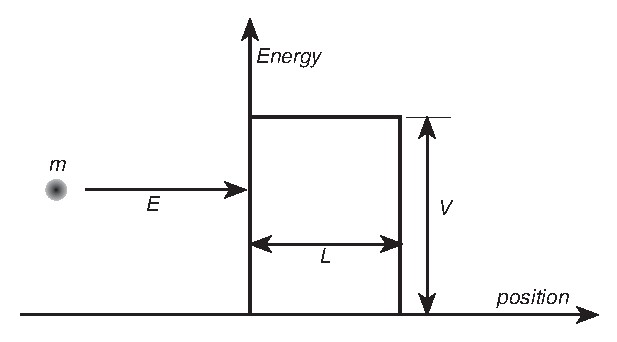
\includegraphics[]{QMBarrier}
% \epsfbox{Pix/QMBarrier.eps}
\end{center}
\caption{One Dimensional Barrier\label{QMBarrier:Fig}}
\end{figure}

This section demonstrates how an algebraic manipulation system might
be used to solve a problem in quantum mechanics that might arise in
practice, or at least in homework.  We wish to determine the
probability that a particle with mass $m$ and energy $E$ will pass
through the one dimension potential barrier given in
\figref{QMBarrier:Fig}.  This probability is called the {\em
transmission coefficient\/}.  We begin with the one dimensional, time
invariant Schr\"odinger equation:
\[
- \frac{\hslash^2}{2 m} \frac{d^2 \psi(x)}{dx^2} + V(x) \psi(x) = E
\psi(x).
\]
Here $\hslash = \frac{h}{2 \pi}$ where $h$ is Planck's constant.  The
mass of the particle is represented by $m$, and the energy by $E$.
The potential energy of the system is $V(x)$ and the wave function of
the particle is $\psi(x)$.

If the potential energy is constant we have
\[
\frac{d^2 \psi(x)}{dx^2} + \frac{2 m\,(E - V)}{\hslash^2} \psi(x) = 0.
\]
All solutions of this equation are linear combinations of two eigenfunctions
of the equations
\[
\psi(x) =  A e^{i \sqrt{2m\,(E - V)} x/ \hslash} + B e^{- i \sqrt{2m\,(E
- V)} x/ \hslash} 
\]
where $A$ and $B$ are arbitrary constants.  The first term in the sum gives
the probability amplitude of motion to the right (increasing $x$), while the
second term corresponds to motion to the left.  

We assume the height of the potential barrier is $V$ and that the
particle has energy $E$ with $E$ greater than $V$.
The barrier has has width $L$ and begins at $x=0$ and goes to
$x=L$.  We need to construct the wave function of a particle moving from
left to right and impinging on the barrier.  In each of the three regimes
$x<0$, $0<x<L$ and $L<x$, the potential is constant and thus the wave
function has the form given above.  We will use continuity conditions to
match the three wave functions at their boundaries.  This allows us to
determine the amplitudes of the wave functions.  We then compute the ratio
of the incoming amplitude and the outgoing amplitude.

We begin by setting two variables {\tt ALPHA} and {\tt BETA} to the wave
numbers of the particle outside the barrier and inside the barrier respectively
\begin{verbatim}
(C1) RADPRODEXPAND:FALSE$
\end{verbatim}
When {\tt RADPRODEXPAND} is set to true, expressions like $\sqrt{a b} /
\sqrt{a}$ will naturally simplify to $\sqrt{b}$ since the numerator will be
represented as $\sqrt{a} \sqrt{b}$.  We have set {\tt RADPRODEXPAND} to
false so that expressions like $\sqrt{2Em}$ will remain a single square
root as is conventional.
\begin{verbatim}
(C2) ALPHA:SQRT(2*M*E)/HBAR;
\end{verbatim}
\mdline{\frac{\sqrt{2Em}}{\hslash}}{D2}
\begin{verbatim}
(C3) BETA:SQRT(2*M*(E-V))/HBAR;
\end{verbatim}
\mdline{\frac{\sqrt{2 m \,(E-V)}}{\hslash}}{d3}
{\tt ALPHA} and {\tt BETA} are the two quantization constants that are
involved in the computation.  We use {\tt HBAR} to represent Planck's
constant.

\begin{verbatim}
(C4) A:1$

(C5) UL:A*%E^(%I*ALPHA*X)+B*%E^(-%I*ALPHA*X);
\end{verbatim}
\mdline{e^{i \sqrt{2Em} x / \hslash} + 
B e^{-{i \sqrt{2Em} x / \hslash}}}{D5}
This is the wave function to the left of the barrier.  Since the 
transmission coefficient is to be the ratio of $|A|^2$ and $|F|^2$, we
set {\tt A} to one here.  By eliminating this variable we reduce the number of
unknown variables to precisely the number of equations obtained by
fitting the pieces of the wave function together.
\begin{verbatim}
(C6) UC:C*%E^(%I*BETA*X)+D*%E^(-%I*BETA*X);
\end{verbatim}
\mdline{C e^{i \sqrt{2m\,(E-V)} x / \hslash}
+ D e^{-i \sqrt{2m\,(E-V)} x / \hslash}}{D6}
The wave function for the regime inside the potential barrier is similar,
but the wave number is different.
\begin{verbatim}
(C7) UR:F*%E^(%I*ALPHA*X);
\end{verbatim}
\mdline{F e^{i \sqrt{2Em} x / \hslash}}{D7}
Beyond the barrier we can assume that there is no reflection of the wave
at infinity.  Thus only one term is needed for the wave function.
\begin{verbatim}
(C8) UL-UC,X=0;
\end{verbatim}
\mdline{-D -C + B +1}{D8}
\begin{verbatim}
(C9) EQ1:%$

(C10) UC-UR,X=L$

(C11) EQ2:%$
\end{verbatim}
Since the wave function is continuous, the various pieces and their
derivatives must match up at the edges of the barrier.
\begin{verbatim}
(C12) EQ3:SUBSTITUTE(0,X,DIFF(UL-UC,X));
\end{verbatim}
\mdline{\frac{i D \sqrt{2 m \, (E-V)}}{\hslash} -
\frac{i C \sqrt{2 m \,(E-V)}}{\hslash} -
\frac{i B \sqrt{2Em}}{\hslash}
+ \frac{i \sqrt{2Em}}{\hslash}}{D12}
\begin{verbatim}
(C13) EQ4:SUBSTITUTE(L,X,DIFF(UC-UR,X))$
\end{verbatim}
These four expressions must be zero for the wave functions to be continuous
and have continuous derivatives.  The expressions are linear in the four
amplitudes, {\tt B}, {\tt C}, {\tt D} and {\tt F}.  Solving this system of
linear equations gives the value of {\tt F}.  We actually want 
the value of {\tt 1/F} since the transmission coefficient is the ratio of
those particles reflected by those which pass through the barrier.
\begin{verbatim}
(C14) SOLVE([EQ1,EQ2,EQ3,EQ4],[B,C,D,F])$

(C18) 1/F,%$
\end{verbatim}
This last quantity is too large to bother printing.  The probability
that particle will pass through the barrier is the magnitude of $F$
which can be determined by $F \overline{F}$, where $\overline{F}$ is the
complex conjugate of $F$.  {\Macsyma} does not have a  function that
computes the complex conjugate of an expression since the conjugate can
be determined by replacing all instances of $i$ in the expression by 
$-i$.  
\begin{verbatim}
(C19) SUBSTITUTE(-%I,%I,%)*%,RATSIMP;
\end{verbatim}
\mdline{\frac{e^{-\frac{2 i L \sqrt{2Em-2mV}}{\hslash}}
\left( 
\begin{aligned}
    \displaystyle
    V^2 e^{4 i L \sqrt{2Em-2mV} / \hslash}\hfill\hfill\hfill\\
    \quad + \left( -2 V^2 + 16EV - 16E^2\right)e^{2 i L \sqrt{2Em-2mV} / \hslash}\\
    \quad +V^2
\end{aligned} \right)}{16EV - 16E^2}}{D19}

The expression given in {\tt D19} is the transmission coefficient desired,
but is certainly not the expression normally given textbooks.  The next few
commands are devoted to simplifying {\tt D19}.  
\begin{verbatim}
(C20) (DEN:PART(%,2),NUM:PART(%,1))$

(C21) RATEXPAND(NUM);
\end{verbatim}
\mdline{
  \begin{aligned}
    V^2 e^{2 i L \sqrt{2Em -2mV} / \hslash}
      &+ V^2 e^{-{2 i L \sqrt{2Em -2mV} / \hslash}}\\
      &-2V^2 +16EV -16E^2
  \end{aligned}}{D21}
We would like to eliminate the complex exponentials.  We could apply
deMoivre's identity to {\tt D19} but a horrible mess of trigonometric
functions would result.  It would be quite difficult to cause {\Macsyma} to
produce the correct answer using that technique.  

The denominator already in roughly the form we would like.  To simplify some
of the steps that follow, we will deal with the numerator and denominators
separately. 
\begin{verbatim}
(C22) D21,DEMOIVRE,RATSIMP;
\end{verbatim}
\mdline{V^2 \left( 2 \cos \frac{2 L \sqrt{2Em -2mV}}{\hslash} -2 \right)
+ 16 EV -16E^2}{D22}

The {\tt DEMOIVRE} command applies deMoivre's identity to {\tt D21}.  By
using {\tt RATSIMP} to simplify the expression the sine terms are caused to
cancel.  The coefficient of $V^2$ has the form $2 \cos 2 \theta - 2$.  We
next use the double angle formula to express {\tt D22} in terms of $\cos
\theta$.

\begin{verbatim}
(C23) ANS:EV(%/DEN,TRIGEXPAND);
\end{verbatim}
\mdline{
  \frac{
    \begin{aligned}
       V^2 \left( 2 \left( \cos^2 \frac{L \sqrt{2Em -2mV}}{\hslash}
         - \sin^2 \frac{L \sqrt{2Em -2mV}}{\hslash}\right) -2 \right)\qquad
         \hfill\\
       \hfill+ 16 EV -16E^2
    \end{aligned}}
    {16EV -16E^2}}{D23}
Unfortunately, {\Macsyma} uses the following double angle identity
\[
\cos 2\theta = \cos^2 \theta - \sin^2 \theta.
\]
By replacing $\cos^2 \theta$ by $1 - \sin^2 \theta$ the expression will be
reduced to a single trigonometric term.  The only problem is picking out
$\theta$.  

The {\tt PART} command in {\Macsyma} is used to out sub-expressions from
a larger expression.  Its first argument is the ``larger expression.''
The second argument says which part to return.  Thus given an
expression like
\[
w = x^2 + (2y - 1) x + 3
\]
{\tt PART($w$, 2)} is second argument to the top level sum, viz.,
$(2y-1) x$.  Successive {\tt PART} commands can be strung together by
additional selectors.  Thus {\tt PART($w$, 2, 1)} is $2y-1$ and so on.

For our problem, the following command will pick out the argument to the
cosine in $D23$.

\begin{verbatim}
(C24) PART(D23,1,1,2,1,2,1,1,1);
\end{verbatim} \mdline{\frac{L \sqrt{2Em - 2mV}}{\hslash}}{D24}
\begin{verbatim}
(C25) SUBSTITUTE(1-SIN(D24)^2,COS(D24)^2,ANS);
\end{verbatim}
\mdline{\frac{V^2
  \left(
    2 \left(1 - 2\sin^2 \frac{2L \sqrt{2Em-2mV}}{\hslash} \right)
    - 2
  \right) + 16EV - 16E^2}{16EV - 16E^2}}{D25}
{\Macsyma} likes to keep expressions as quotients of polynomials.  In this case
we would prefer to see the answer as $1 + <\hbox{quotient of polynomials}>$.
The following command does that. 
\begin{verbatim}
(C26) 1+FACTOR(RATSIMP(D25-1));
\end{verbatim}
\mdline{\frac{\sin^2 \left(\frac{L \sqrt{2M (E - V)}}{\hslash}\right) V^2}{4E(E-V)} +1}{D26}
Thus the transmission coefficient for a particle impinging on a potential
barrier of height $V$ is
\[
1 + \frac{\sin^2 \frac{L \sqrt{2 m\,(E - V)}}{\hslash} V^2}{4 E \, (E - V)}.
\]
which is what we normally find in textbooks.

\section{Overview of the Algorithms and Capabilities}

As can be seen from these examples, algebraic manipulation systems can deal
directly with many of the quantities that arise in mathematics:
polynomials, rational functions, matrices and power series, for example.
Basic arithmetic operations with these types of objects can be implemented
relatively straightforwardly, however numerous performance complications
arise because of {\em intermediate expression swell\/}.  Arithmetic
operations with symbolic quantities tend to produce larger expressions from
smaller ones.  This distinguishes symbolic calculations from numeric ones
where numeric expressions tend not to grow in size.  Intermediate
expression swell occurs in a problem when the intermediate computations
swell to be much larger than the final answer.  A prime example of this
problem occurs when calculating polynomial GCD's.  These issues are
discussed in some detail in \chapref{Poly:Arith:Chap} and some approaches
to their solution are given in Chapters \ref{Interpolation:Chap} and
\ref{Hensel:Chap}. 

Symbolic systems are more likely to deal with infinite structures such as
ideals, lattices or power series, than numerical systems.  We want to perform
the same types of operations on these structures as on simpler structures.
In \chapref{Ideal:Arithmetic:Sec}.

There are certain additional operations that are possible with symbolic
quantities.  \rightmarginnote{orthogonal functions expansions, analysis of
singularities} 
Some operations that are impractical for numerical quantities
turn out to be quite cheap for symbolic expressions.  For instance,
there is no known polynomial time algorithm for factoring integers, and
more to the point it is quite hard in practice to factor integers.
However, there do exist polynomial time algorithms for factoring
polynomials, and in practice polynomials are relatively easy to
factor.\footnote{The distinction between practice and theory is made here
because the polynomial time algorithm is an $O(n^{12})$ algorithm, while
the exponential algorithms which are used in practice  usually only 
require $O(n^{3})$ operations.}

Another	aspect of symbolic computation is exact versus inexact computation.

Where there are similarities between numerical and symbolic calculations,
the introduction of symbolic parameters often allows one to examine a wide
variety of possibilities with a single computation.

Groups, Fields, Riemann surfaces, topological structures, etc as first
class objects.

Computations: arithmetic, solving systems of equations, approximation
techniques, etc.


Problems: simplification: definite canonical and normal simplifiers.




\section{Where Current Research is Heading}

With some exceptions the contents of this book are largely classical.
The algorithms discussed are solutions to the problems set out by
parents of the Computer Algebra field at the end of the 1960's.  Since
then, much has changed.  The massive increase in performance of computer
systems and their precipitative drop in price has changed many of the
premises upon which computer algebra research is based.

